%! Author = Len Washington III
%! Date = 2/3/24

% Preamble
\documentclass[assignment={2},
duedate={Sunday, February 11, 2024, 11:59 PM CST},
points={30}]{cs581homework}

\newcolumntype{P}[1]{>{\centering\arraybackslash}p{#1}}
\newcommand{\heading}[1]{\textcolor{white}{\textbf{#1}}}
\newcommand{\bigram}[4]{%
	Probability of a sentence:
	\begin{center} \emph{#1} \end{center}
	\begin{table}[H]
	    \centering
		\label{tab:}
		\begin{tabular}{|p{0.75\textwidth}|}
			\hline
			\textbf{Relevant bigram \textcolor{red}{probabilities} [1 pt]:}\\
			\hline
			#2\\
			\hline
			\textbf{Probability of a sentence formula [2 pt]:}\\
			\hline
			#3\\
			\hline
			\textbf{Probability of a sentence (calculations and value) [2 pt]:}\\
			\hline
			#4\\
			\hline
		\end{tabular}
	\end{table}

}

% Document
\begin{document}

\maketitle

\begin{objectives}
	\begin{enumerate}
	    \item (10 points) Demonstrate your understanding of Minimum Edit Distance algorithm.
	    \item (10 points) Demonstrate your understanding of the N-gram language modeling.
	    \item (10 points) Demonstrate your understanding of an HMM POS tagger.
	\end{enumerate}
\end{objectives}

\problem[10]{1}
What is the \textbf{Minimum Edit Distance} between words STALK and FABLE (assume that insertion / deletion cost is 1, substitution cost is 2)?
Populate the table below to find the MED\@.
Include back pointers.

\begin{table}[H]
    \centering
	\label{tab:med}
	\begin{tabular}{|*{7}{P{0.12\textwidth}|}}
		\hline
		\textbf{K} &  &  &  &  &  &  \\
		\hline
		\textbf{L} &  &  &  &  &  &  \\
		\hline
		\textbf{A} &  &  &  &  &  &  \\
		\hline
		\textbf{T} &  &  &  &  &  &  \\
		\hline
		\textbf{S} &  &  &  &  &  &  \\
		\hline
		\textbf{\#} &  &  &  &  &  &  \\
		\hline
		& \textbf{\#} & \textbf{F} & \textbf{A} & \textbf{B} & \textbf{L} & \textbf{E} \\
		\hline
	\end{tabular}
\end{table}

\problem[10]{2}
Your task is to calculate probabilities of selected sentences in English using a language model (based on Google Books N-gram corpus).
Use the Google N-Gram Viewer website \url{https://books.google.com/ngrams} to collect all necessary data
(NOTE: Google provides N-gram \textcolor{red}{PERCENTAGES} - \textcolor{red}{those are NOT COUNTS! and not exactly probabilities!}) and calculate sentence probability.

\begin{figure}[H]
	\centering
	\caption{Notes: \\ - assume that probability of any bigram starting or ending a sentence is 0.25. \\ - use the settings shown below (2018 probabilities, English (2019), case insensitive, Smoothing of 1)}
	\label{fig:}
	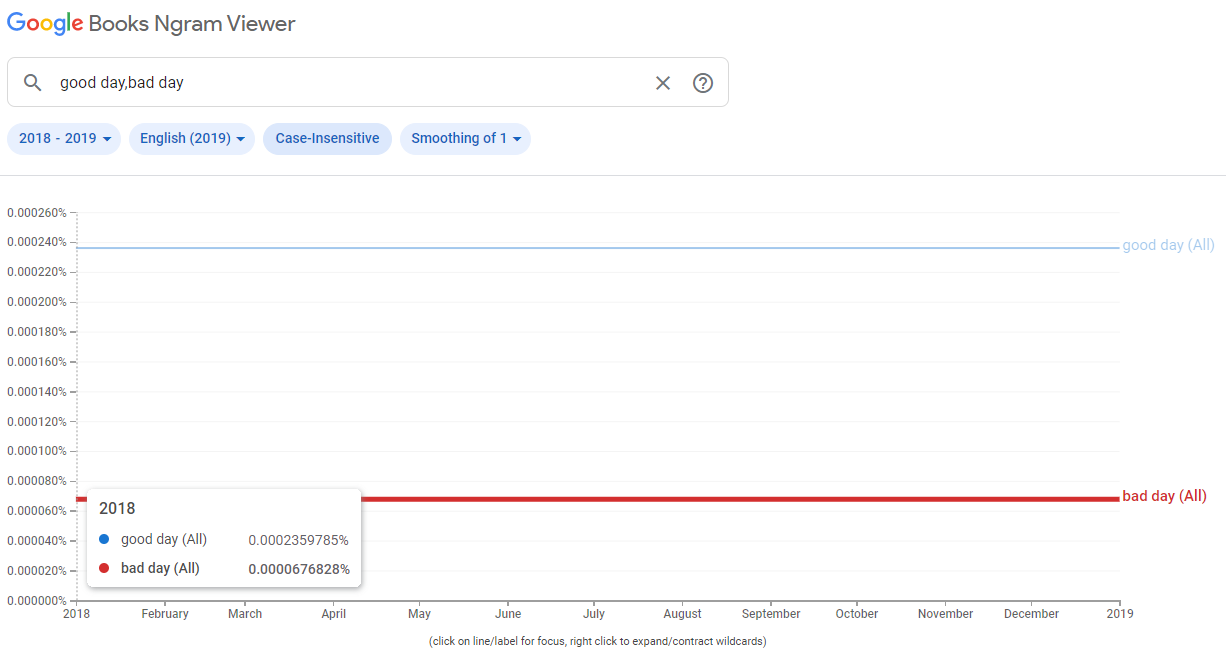
\includegraphics[width=\textwidth]{ngram}
\end{figure}

A) \bigram{Today is a good day}{~}{~}{~}
B) \bigram{Today is a bad day}{~}{~}{~}

\problem[10]{3}
Given the following Hidden Markov model (transition probabilities shown; emission probabilities to be determined by you using corpus $C$ data) based on corpus $C$:

\begin{figure}[H]
	\centering
	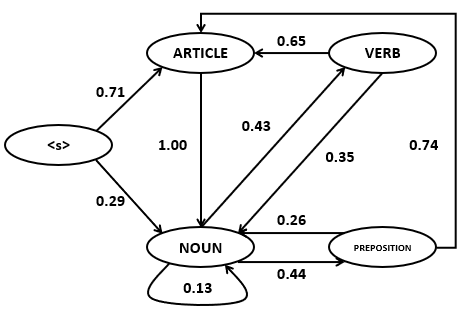
\includegraphics[width=\textwidth]{hmm}
	\label{fig:hmm}
\end{figure}

And the following table of selected word counts from some corpus $C$:
\begin{table}[H]
    \centering
	\label{tab:corpus}
	\begin{tabular}{|*{6}{0.16\textwidth}}
		\rowcolor{black} \heading{Word/Tag} & \heading{N} & \heading{V} & \heading{Art} & \heading{P} & \heading{Total}\\

	\end{tabular}
\end{table}



\end{document}